\chapter{Waypoints positioning} 
\minitoc
To remind, the main objective is to propose a efficient path to can cover an area using a camera mounted on a UAV. In the solution proposed here is to in the first time, focus on optimize the position of a cameras set to fully cover an area. When a optimized position of the cameras set is found the position can be used as waypoints for an UAVs path. Indeed find an optimized position for each camera of a given set is primordial. The following section are dedicated to the optimization of it in order to have an efficient solution to place the waypoints.




%\section{An optimization problem.}

During the previous section the problem was already discussed as an optimization problem. The formulation of the problem was presented to can apply some optimization problems and also the complexity of the problem was disused in the section \ref{sec:OptimizationComplexity}.



\section{PSO. }

The PSO (Particle Swarm Optimization) is an algorithm dedicated to the optimization problems. It is an stochastic algorithms form the family of evolutionary algorithms (see \ref{chap:EA}). 
The PSO is a relatively young compared then the other EA. It was developed by Russel Eberhart and James Kennedy in 1995 [148* bis]. The concept of PSO is to optimize iteratively a continuous non linear function. To do that the PSO is inspired by the behaviour of animals. As it append here form the bird flocking, fish schooling and swarming theory. These animals working in group to find food. 
The direction to take is not decide by one leader, but by all individuals of the swarm by relaying just few informations as what quantities of food their found. 
The swarm composed by numerous individuals became smarter and more efficient to reach their objective. 
The algorithm proposed by Russel Eberhart and James Kennedy in [148* bis] are directly inspired by these behaviours.

The methodologies used is to consider each individual or also called particles as a solution of the problems. The problems is optimized at each iteration. To do that each solution must be comparable and quantifiable. At each iteration, each particle have to be tested by a cost function in order to discriminate the best particles of the swarm. The cost function and the design of it has been detailed in the section \ref{chap:formulation}.
When the best particle is found at the end of an iteration, the other particles of set try to change their initial direction to converge more or less quickly to the actual best. 
Indeed the power of this algorithm is to have a very basic individuals behaviour to guide the particles. 
Each particles are guided by 3 behaviours.
 \begin{itemize}
 \item  This own velocity $V_k$. 
 \item  This own best solution $P_i$.
 \item  The best solution $P_g$.
\end{itemize}  
Here the velocity represent the useful speed of the particle to converge to the best solution. More the velocity is high more the step at each iteration will be long. 
The behaviour of the particles $X_k$ are modelled by the following equation to obtain the new position $X_{k+1}$ :
\begin{equation} \label{eq:PSO}
\begin{split}
 V_{k+1}= \omega V_k +b1(P_i -X_k)+b2(P_g-X_k)
\\
\mbox{ and } \\ X_{k+1}=X_k+V_{k+1}
\end{split}
\end{equation}

Where $\omega$ is the inertia. $b1$ is random value between 0 and $\phi_p$ and $b2$ is random value between 0 and $\phi_g$. $\phi_g$ and $\phi_p$  are the scaling factor to search away from the particles is best known position (Default: 0.5). 

Thanks to this basic behaviour of the particles the swarm can coverage to an global solution. 
To have an efficient optimization just few parameters must be set-up for the PSO.  
The more important are the inertia of the particles, the size of the swarm and the initial dispersion.
\begin{itemize}
\item The inertia  will globally  help the particles to keep  their  initial velocity. The consequences of the high value of inertia is to explore more the search space and therefore the convergence will be longer. 
\item The size of the swarm  have an impact on the convergence time (in number of iteration) and the also time computation. Indeed a big amount of particles in the swarm  mean more exploration of the search space at each iteration, but also more comparison to find the best particles (the comparison may have a non negligible computation time). 
The swarm size is commonly fixed but can be as the population in the GA (see section \ref{sec:Population} ) dynamically adjusted during the optimization process. 


\item The initial dispersion of the swarm can be a decisive element as the population for the GA (see in \ref{sec:initPOP}). For the PSO the use of an heuristic to initialize all the particles of the swarm is not recommended due to this important risk to converge prematurely in a local minimum. The random dispersion appear  as the more appropriate. 
\item Other criteria as $\phi_g$ and $\phi_i$ are minor but can be useful to fine adjust the PSO.
\end{itemize}

Finally to summarize the PSO is efficient in term of optimization despite a very basic behaviour of each particles. Each particles have this own velocity defined part way by the random and controlled by a global parameters the inertia.
 The power of PSO is at same time this efficiency to solve the optimization problem and this simplicity of use. In fact the PSO need at minima  few element to work properly : a cost function, an inertia parameters and the size of the swarm. These efficiency and simplicity of use explain this popularity during the last decade.
 





-the initial dispersion of the particles \\
%- size swarm \\
%- stopping criteria \\
- inconvenient 


\section{Random selection }
PSO camera position 
8 33 87 84 143(transitor) 193 194 200(capter 360)201
148 origine de PSO. 
PSO[84 8 33 143] 87 193* 194* 200* 201* 

228*(hibrid) 161* 158* 78 GA VS PSO

\section{GA VS PSO }\label{sec:GAvsPSO} 
%

\begin{mfigures}{For the experiments: (a), (b), (c) the blue rectangle represents the field of view of one camera projected onto the ground  with z=1 ($30 \times 20 $px) and (d), (e) with z=2 ($60 \times 40 $px)}{fig:Rooms_shapes} \centering
\mfigure{width=.4\linewidth}{img/fig7-a.png}{Simple room}{subfig:r1}
\hspace{1cm}
\mfigure{width=.4\linewidth}{img/fig7-b.png}{Big room}{subfig:r2}
\mfigure{width=.4\linewidth}{img/fig7-c.png}{Room U}{subfig:r3}
\hspace{1cm}
\mfigure{width=.4\linewidth}{img/fig7-d.png}{Room L}{subfig:r4}
\mfigure{width=.4\linewidth}{img/fig7-e2.png}{Big room L}{subfig:r5}
\end{mfigures}

To find the best coverage, many experiments have been used to compare PSO and GA. PSO is easier to implement and runs faster, but GA is more flexible and generic thanks to the many tunable parameters. 
The following subsections will provide a comparison between PSO and GA and give an overview of our method, which is based on GA. The comparison demonstrates the overall advantage of the latter over the former.\\
In the literature, the PSO was often used \cite{8*zhou2011,33*reddy2012}, mostly because of the simplicity of its implementation. However, it is interesting to compare the algorithm with the GA. The two algorithms are from the same family (both are stochastic and from evolutionary algorithms).\\
To compare and evaluate their performance, we tested them in different scenarios depicted in Figure \figref{fig:Rooms_shapes}, with areas  of different size and shapes, where: 




\begin{itemize}
\item[-]    z is the height of the camera between (within the range $[1/z;z]$).
\item[-]	Figure \figref{subfig:r1} is an area of size 120$\times$80 (named Room). 
\item[-]	Figure \figref{subfig:r2} is an area of size 240$\times$160 (named Big Room).
\item[-]	Figure \figref{subfig:r3} is an area of size 120$\times$80 (named Room U).
\item[-]	Figure \figref{subfig:r4} is an area of size 120$\times$80 (named Room L).
\item[-]	Figure \figref{subfig:r5} is an area of size 240$\times$80 (named Big Room L).
\end{itemize}


The design of the experiments in Table \ref{table:table1} has been set up to identify the most efficient algorithm for the positioning of a set of waypoints with maximum coverage. 

\begin{table}[!htb]
\begin{tabular}{|l|l|l|l|l|l|}
  \hline
  \multicolumn{2}{|l|}{z=1 } &\multicolumn{2}{|c|}{GA}  & \multicolumn{2}{|c|}{PSO} \\  \hline
  \multicolumn{2}{|c|}{ } & GT & NW & GT & NW\\ \hline
  Room &  120x80 & 16 &20 & 16 & 20\\ \cline{2-6}
     &  240x160 & 64 &70 & 64 & 70 \\ \hline
  Room U &  120x80 & 12 &20 & 12 & 20\\ \hline
  \multicolumn{2}{|l|}{z=2 } &\multicolumn{2}{|c|}{GA}  & \multicolumn{2}{|c|}{PSO} \\  \hline
 Room &  120x80 & 4 &10 & 4 & 10\\ \cline{2-6}
     &  240x160 & 16 &20 & 16 & 20 \\ \hline
 Room L&  120x80 & 3 &10 & 3 & 10\\ \cline{2-6}
     &  240x160 & 15 &20 & 15 & 20 \\ \hline
\end{tabular}
\caption{Design of the experiment for comparing the efficiency of PSO and GA in different conditions.  (GT is Ground Truth and NW is Number of Waypoints).}\label{table:table1}
\end{table}

The Ground Truth (GT) is the minimum number of waypoints required to fully cover a given area. The size of the area has been selected so that the GT can be easily estimated. 

NW is the maximum Number of Waypoints (or camera views) used for the experiments.  
At each experiment a solution is computed for a number of waypoints from 1  to NW. To compare the different algorithms fairly, only 10 000 calls of the cost function are allowed for each set of waypoints.\\

\subsubsection{ Analysis of the result.}

After performing the experiments (see Table \ref{table:table1}), it appears that the GA and PSO algorithms are close in performance. In some cases, GA is much more efficient (see Figure \ref{fig:bigRz1}) particularly in the case where the search space is large (big room and big number of cameras),  as the example in Figure \ref{fig:bigRz1}. Instead, PSO is more effective for optimizing small areas (see Figure \ref{fig:RLz2} ).
This efficiency can be explained by the small variation of the solution introduced by the PSO. 

However, this small variation is not enough to find an optimized solution in a big search space that occurs when many cameras are required or when the local minimum is deeper.
Although the variety of solutions introduced by the GA allows the escape from local minima, it can negatively affect the accuracy of the solution and may require a further optimization step to refine. 

%\begin{figure}
%\minipage{0.99\textwidth}
%  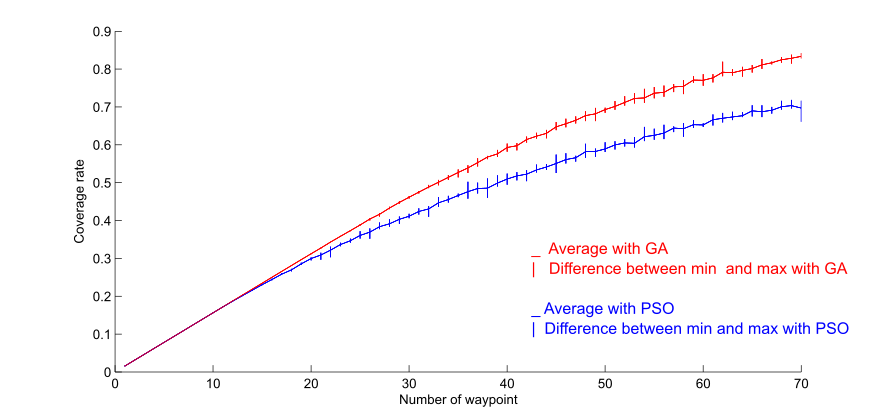
\includegraphics[width=\linewidth]{img/fig8.png}
%  \caption{ Comparison of eight solutions given by the GA, with eight solutions given by PSO algorithms with a fixed altitude ($z$ equal to 1) in the big room 240x160. The ground truth for this room equals to 64.}\label{fig:bigRz1}
%   \endminipage\hfill
%\end{figure}
%
%
%\begin{figure}
%\minipage{0.99\textwidth}
%  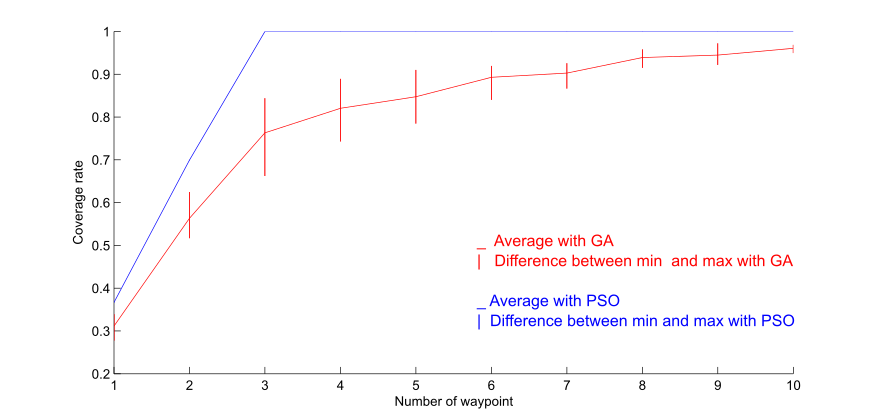
\includegraphics[width=\linewidth]{img/fig9.png}
%  \caption{Comparison of eight solutions given by the GA, with eight solutions given by PSO algorithms with a Z between [1/2; 2] in the room with L shape 120x80 and ground truth equal to 15.}\label{fig:RLz2}
%   \endminipage\hfill
%\end{figure}

 Following the comparison of the 2 algorithms, the GA seems more suited for finding UAV waypoints especially if it navigates in a large room or an outdoor scene.
Furthermore, our comparative study demonstrates that the GA is less dependent on the shape of the area to cover. \\
According to the previous results, the genetic algorithm will be used during future work with no restriction at the convergence point to optimize the positioning of the waypoints in the bigger areas seen in Section  \ref{coverageOutDoor} such as in Figure \ref{subfig:satimg+mask}.\\


fill with the jirs 
	\subsection{DoF Design of Experiment}
	\subsection{Result}
	\subsection{Explication}

\section{Hybrid GA PSO}
 76* 77* 78*
	\subsection{memetic ???}
		\subsubsection{DoF}
		\subsubsection{Result}
		\subsubsection{Conclusion}
		
\section{Experiment}
	\subsection{No obstacle }
	\subsection{Rectangle obstacle}
	\subsubsection{With mask}
	\subsection{For big area}
		\subsubsection{map 1}
		\subsubsection{map2 torcy}
		\subsubsection{map3 calvisson}
		


%%%%%%%%%%%%%%%%%%%%%%%%%%%%%%%%%%%%%%%%%%%%%%%%%%%%

 


